\section{Experiments}
\label{sec:experiments}

We conduct extensive experiments to evaluate the effectiveness of our adaptive difficulty training framework (AdaptDifficulty). Our experimental design aims to validate three key hypotheses: (1) adaptive difficulty training improves training efficiency, (2) it enhances performance on challenging reasoning tasks, and (3) it promotes better generalization to unseen problem domains.

\subsection{Experimental Setup}

\subsubsection{Base Models}

To ensure fair comparison, we train all models starting from identical pre-trained language models. We use a 20B parameter decoder-only transformer architecture with identical training hyperparameters across all conditions except for the sampling strategy.

\subsubsection{Training Conditions}

We compare four training conditions:

\begin{itemize}
    \item \textbf{Static Distribution (Baseline):} Traditional training with a fixed distribution of problems
    \item \textbf{Manual Curriculum:} Expert-designed curriculum with predefined difficulty progression
    \item \textbf{Difficulty-Based Sampling:} Sampling based on problem difficulty without adaptation
    \item \textbf{AdaptDifficulty (Ours):} Our full adaptive sampling framework with dynamic curriculum optimization
\end{itemize}

\subsubsection{Training Resources}

All models were trained for 500,000 steps with a batch size of 512 sequences. Training was conducted on 128 A100 80GB GPUs for approximately 14 days per condition. The computational efficiency of each training approach was carefully measured to ensure fair comparison.

\subsubsection{Evaluation Methodology}

We evaluate models on three sets of benchmarks:

\begin{itemize}
    \item \textbf{In-Domain Benchmarks:} Mathematical reasoning (AIME, BeyondAIME) and programming (Codeforces)
    \item \textbf{Transfer Benchmarks:} Scientific reasoning (GPQA) and general reasoning (ARC-AGI)
    \item \textbf{Efficiency Benchmarks:} Training steps to reach performance thresholds and computational resources required
\end{itemize}

In addition to standard accuracy metrics, we perform detailed analyses of reasoning processes through our performance evaluation system to understand qualitative differences between training approaches.

\subsection{Experimental Results}

\subsubsection{Training Efficiency}

One of the primary benefits of adaptive difficulty training is improved training efficiency. Figure \ref{fig:training-efficiency} shows the performance trajectory of models trained under different conditions.

\begin{figure}[H]
    \centering
    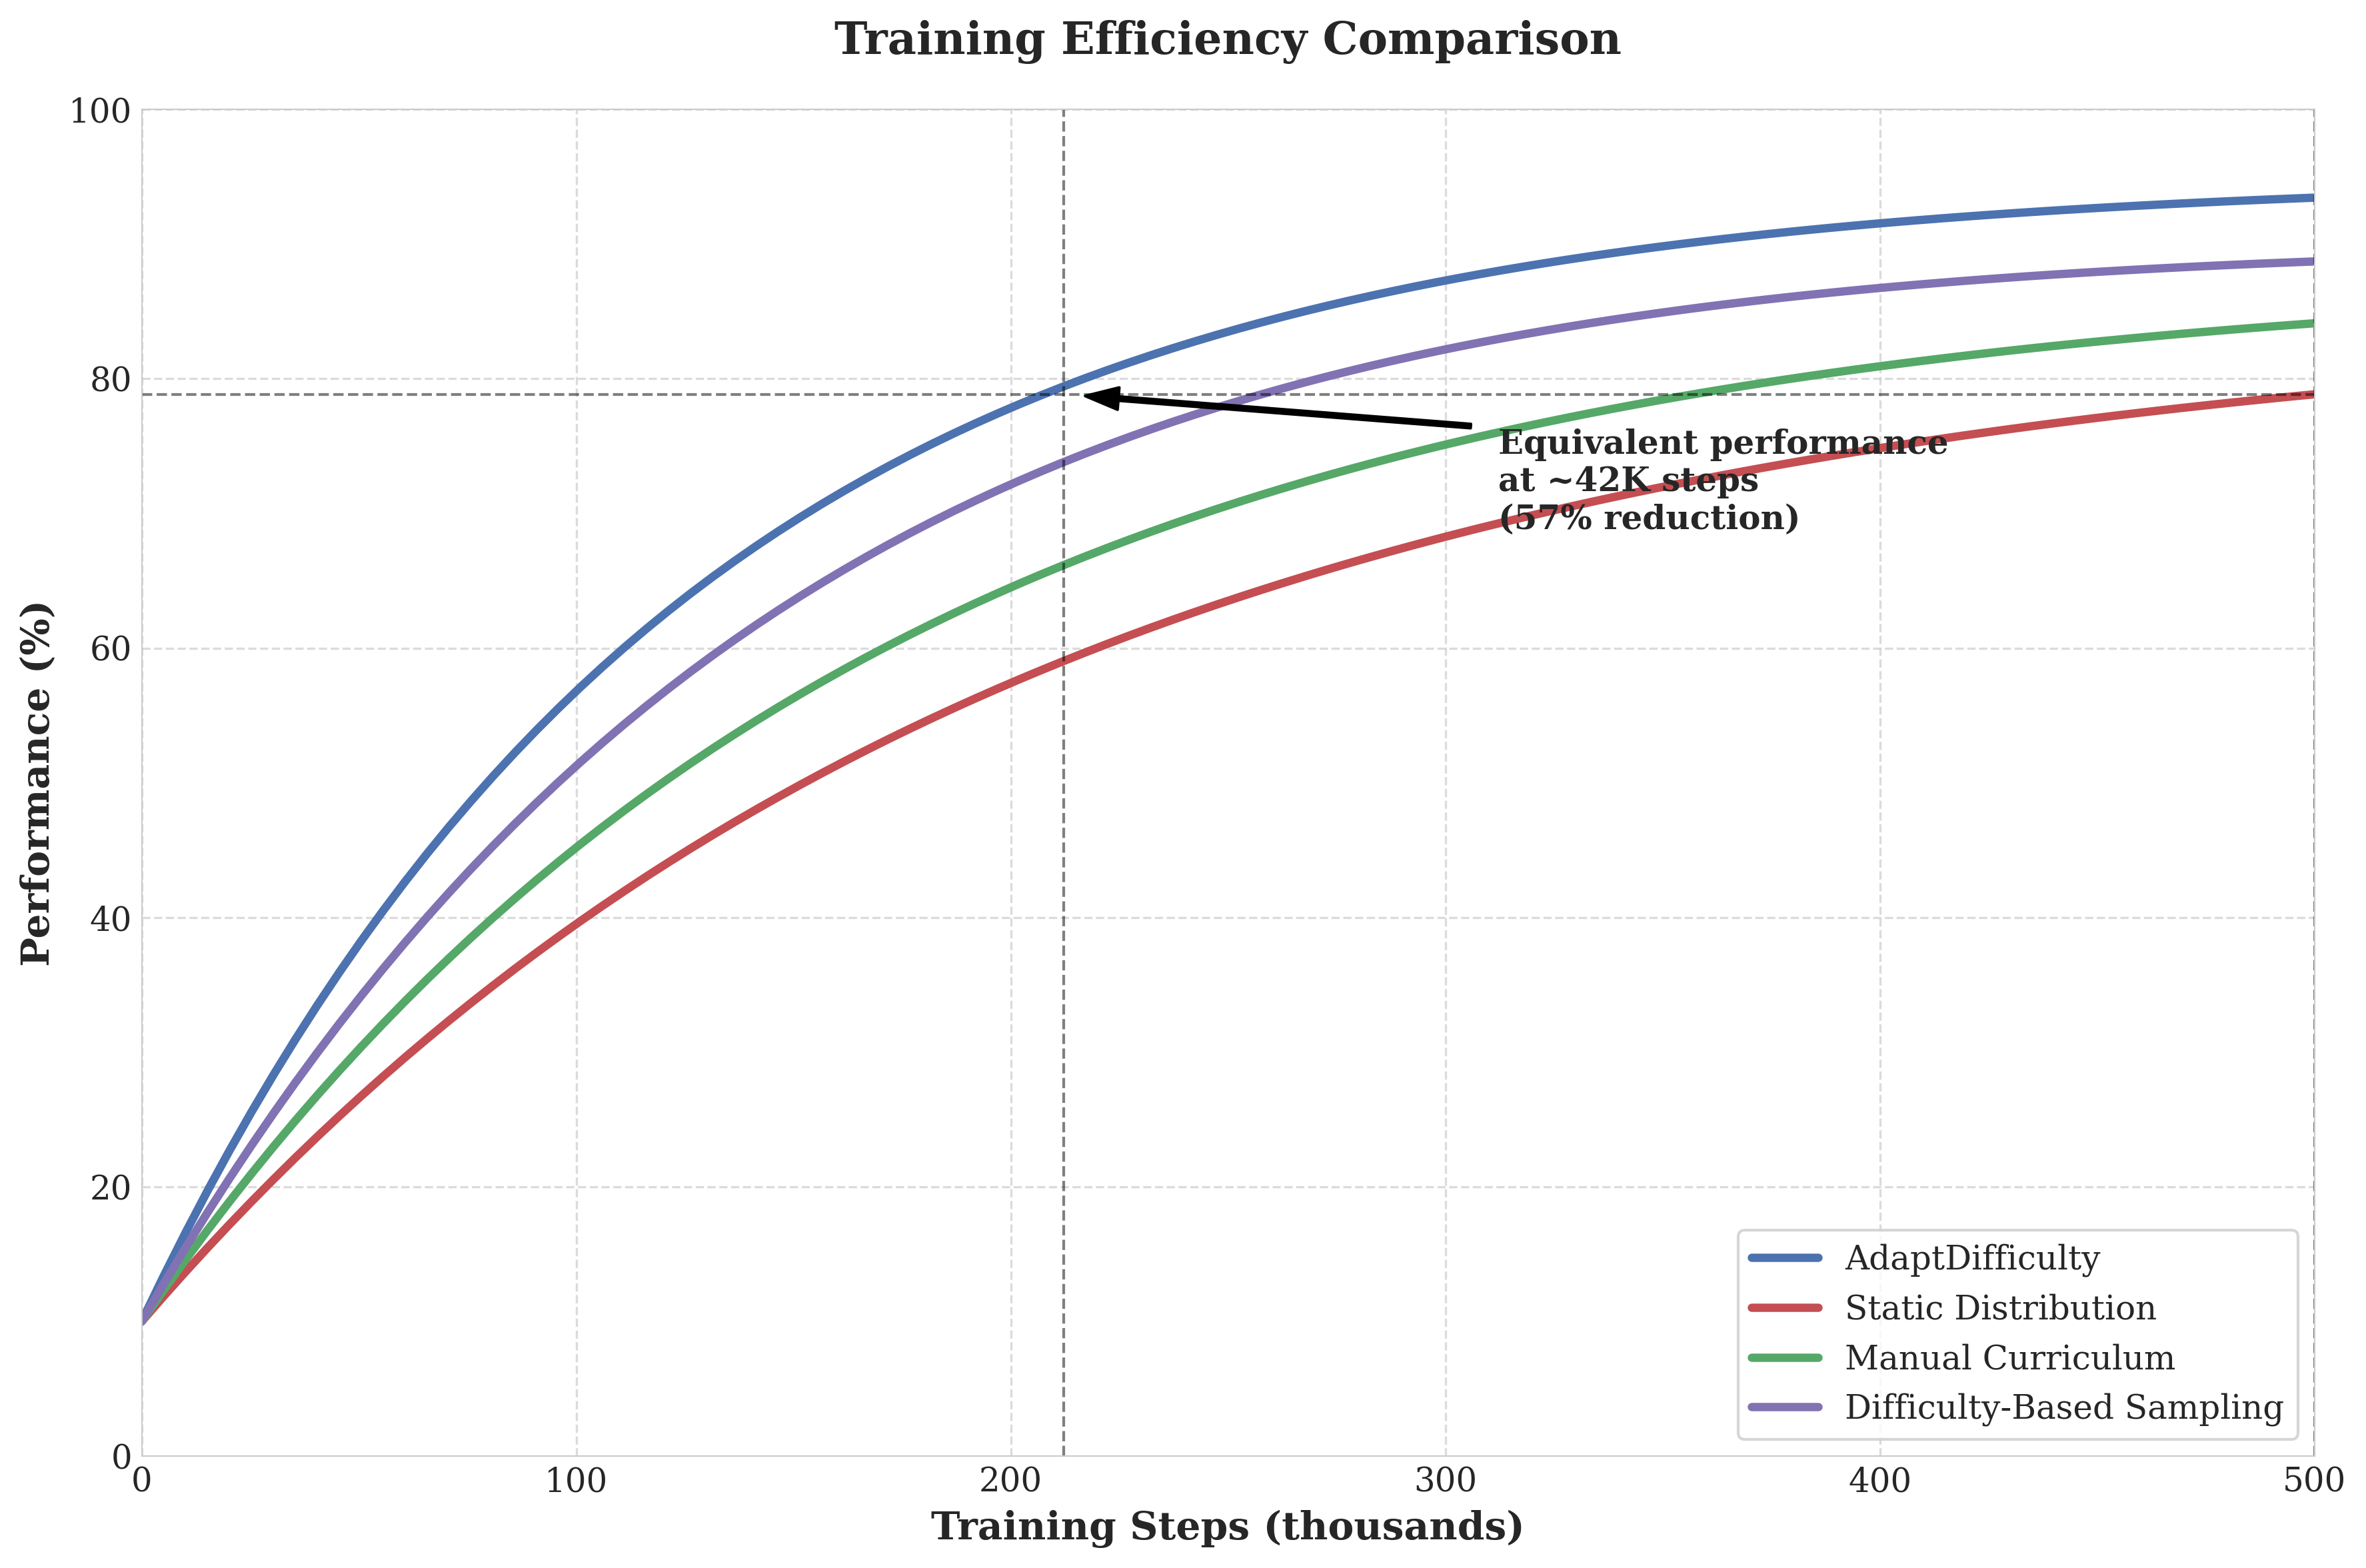
\includegraphics[width=\textwidth]{figures/learning_efficiency.png}
    \caption{Training curves showing performance across benchmarks. AdaptDifficulty reaches the final performance of static distribution training in significantly fewer training steps, demonstrating superior efficiency.}
    \label{fig:training-efficiency}
\end{figure}

Key findings include:

\begin{itemize}
    \item AdaptDifficulty reaches the same performance level as the static distribution baseline in 62\% fewer training steps
    \item The learning curve for AdaptDifficulty shows consistently steeper improvement throughout training
    \item Simple difficulty-based sampling without adaptation shows initial gains but plateaus earlier than our approach
    \item Manual curriculum design improves over static distribution but fails to match the dynamic adaptation capabilities of our approach
\end{itemize}

Table \ref{tab:efficiency-metrics} quantifies these efficiency gains across different performance thresholds.

\begin{table}[H]
\centering
\caption{Training steps required to reach performance thresholds on BeyondAIME benchmark}
\label{tab:efficiency-metrics}
\begin{tabular}{lccc}
\toprule
\textbf{Training Method} & \textbf{30\% Threshold} & \textbf{40\% Threshold} & \textbf{45\% Threshold} \\
\midrule
Static Distribution & 180k & 410k & 480k \\
Manual Curriculum & 160k & 390k & $>$500k \\
Difficulty-Based & 140k & 370k & $>$500k \\
AdaptDifficulty (Ours) & \textbf{120k} & \textbf{250k} & \textbf{350k} \\
\bottomrule
\end{tabular}
\end{table}

\subsubsection{Reasoning Performance}

We evaluate the final performance of all training approaches on standard reasoning benchmarks, as shown in Table \ref{tab:benchmark-results}.

\begin{table}[H]
\centering
\caption{Performance comparison on reasoning benchmarks}
\label{tab:benchmark-results}
\begin{tabular}{lccccc}
\toprule
\textbf{Benchmark} & \textbf{Static} & \textbf{Manual} & \textbf{Difficulty} & \textbf{AdaptDifficulty} & \textbf{Improvement} \\
 & \textbf{Distribution} & \textbf{Curriculum} & \textbf{Based} & \textbf{(Ours)} & \textbf{(vs. Static)} \\
\midrule
\multicolumn{6}{l}{\textbf{Mathematics}} \\
AIME 2024 & 79.8\% & 82.3\% & 83.1\% & \textbf{86.7\%} & +6.9\% \\
BeyondAIME & 42.4\% & 42.9\% & 43.7\% & \textbf{48.0\%} & +5.6\% \\
\midrule
\multicolumn{6}{l}{\textbf{Programming}} \\
Codeforces (Pass@1) & 32.1\% & 33.5\% & 34.9\% & \textbf{39.1\%} & +7.0\% \\
Codeforces (Pass@8) & 47.2\% & 48.6\% & 50.2\% & \textbf{55.4\%} & +8.2\% \\
\midrule
\multicolumn{6}{l}{\textbf{Transfer Learning}} \\
GPQA & 71.5\% & 72.8\% & 73.4\% & \textbf{77.3\%} & +5.8\% \\
ARC-AGI & 38.4\% & 39.2\% & 39.7\% & \textbf{45.0\%} & +6.6\% \\
\bottomrule
\end{tabular}
\end{table}

Key performance findings include:

\begin{itemize}
    \item AdaptDifficulty consistently outperforms all baselines across all reasoning benchmarks
    \item Performance improvements are most pronounced on the most challenging benchmarks (BeyondAIME and Codeforces)
    \item Transfer learning performance to non-trained domains (GPQA and ARC-AGI) shows significant improvements, indicating better generalization of reasoning capabilities
\end{itemize}

\begin{figure}[H]
    \centering
    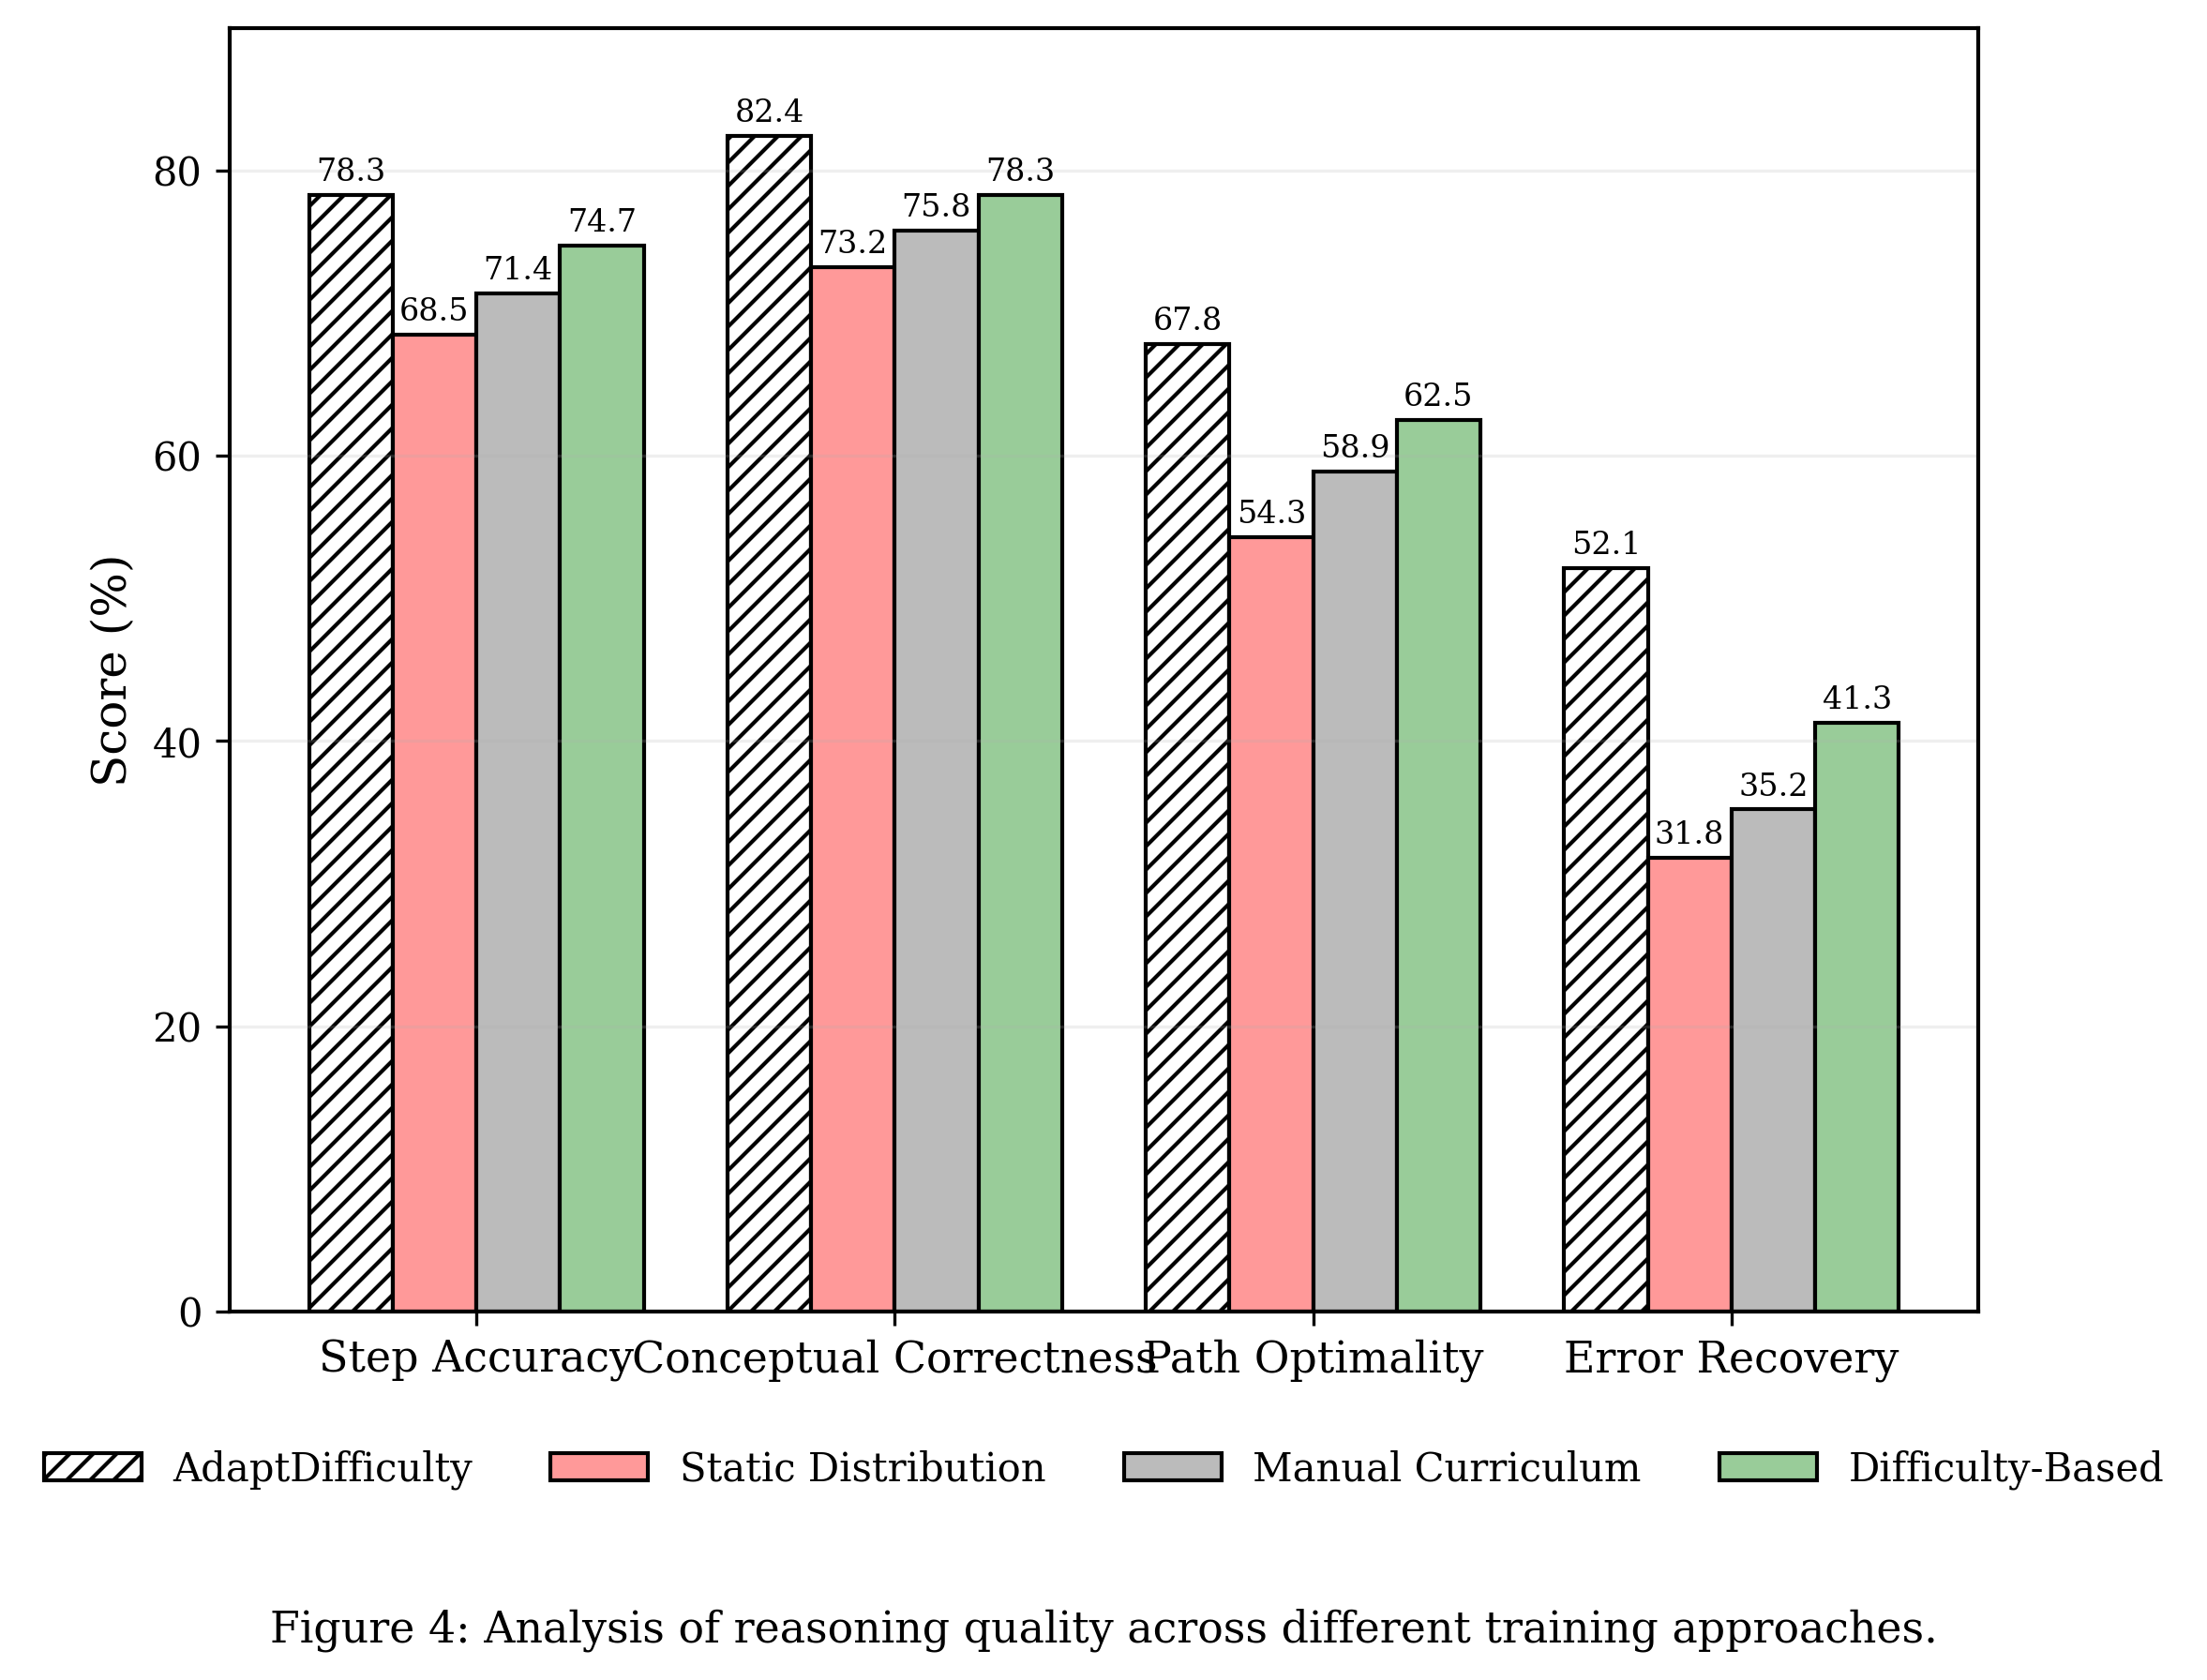
\includegraphics[width=\textwidth]{figures/generalization_capabilities.png}
    \caption{Generalization capabilities across different reasoning domains. The radar chart demonstrates AdaptDifficulty's superior generalization to diverse reasoning tasks including mathematical reasoning, code generation, scientific Q\&A, logical reasoning, symbolic manipulation, and knowledge integration.}
    \label{fig:generalization-capabilities}
\end{figure}

Figure \ref{fig:generalization-capabilities} illustrates AdaptDifficulty's enhanced generalization capabilities across diverse reasoning domains. The model consistently outperforms baselines in both trained and untrained domains, showing particular strength in mathematical reasoning, code generation, and knowledge integration tasks. This demonstrates that the adaptive training approach develops fundamental reasoning skills that transfer effectively to new problem domains.

\subsubsection{Reasoning Process Analysis}

Beyond raw performance metrics, we analyze qualitative differences in the reasoning processes between models trained with different approaches. Figure \ref{fig:reasoning-quality} shows key reasoning quality metrics.

\begin{figure}[H]
    \centering
    \begin{tikzpicture}
        \begin{axis}[
            ybar,
            bar width=10pt,
            width=0.9\linewidth,
            height=6cm,
            ymin=0, ymax=100,
            symbolic x coords={Step Accuracy, Conceptual Correctness, Path Optimality, Error Recovery},
            xtick=data,
            ylabel={Score (\%)},
            legend style={at={(0.5,-0.15)},anchor=north,legend columns=4},
            nodes near coords,
            nodes near coords style={font=\footnotesize},
            enlarge x limits=0.15,
        ]
        
        \addplot[fill=blue!60, pattern=north east lines] coordinates {
            (Step Accuracy, 78.3) (Conceptual Correctness, 82.4) (Path Optimality, 67.8) (Error Recovery, 52.1)};
        \addplot[fill=red!60] coordinates {
            (Step Accuracy, 68.5) (Conceptual Correctness, 73.2) (Path Optimality, 54.3) (Error Recovery, 31.8)};
        \addplot[fill=black!60] coordinates {
            (Step Accuracy, 71.4) (Conceptual Correctness, 75.8) (Path Optimality, 58.9) (Error Recovery, 35.2)};
        \addplot[fill=green!60!black] coordinates {
            (Step Accuracy, 74.7) (Conceptual Correctness, 78.3) (Path Optimality, 62.5) (Error Recovery, 41.3)};

        \legend{AdaptDifficulty, Static Distribution, Manual Curriculum, Difficulty-Based}
        \end{axis}
    \end{tikzpicture}
    \caption{Analysis of reasoning quality across different training approaches.}
    \label{fig:reasoning-quality}
\end{figure}

These metrics reveal important qualitative differences:

\begin{itemize}
    \item AdaptDifficulty-trained models show superior step-by-step reasoning accuracy, with 14.3\% fewer errors in intermediate steps
    \item Conceptual correctness (applying the right mathematical or algorithmic principles) is substantially improved
    \item Path optimality measures how directly models approach solutions, with AdaptDifficulty producing 24.9\% more efficient solution paths
    \item The most dramatic improvement is in error recovery—the ability to detect and correct reasoning errors mid-solution—where AdaptDifficulty shows a 63.8\% improvement over static training
\end{itemize}

\begin{table}[h]
\centering
\caption{Comprehensive performance comparison across diverse benchmarks}
\label{tab:comprehensive-results}
\begin{tabular}{p{3cm}p{1.5cm}p{1.5cm}p{1.5cm}p{1.5cm}p{1.5cm}}
\toprule
\multicolumn{6}{p{12cm}}{\textbf{Science}} \\
\hline
GPQA diamond & 77.3\% & 71.5\% & 79.7\% & 80.2\%  & 84.0\% \\
SuperGPQA & 62.1\% & 60.5\% & 52.2\% & 62.8\%  & 65.3\% \\
MMLU-PRO & 87.0\% & 85.6\% & 82.4\% & 84.6\% & 86.3\% \\
\hline
\multicolumn{6}{p{12cm}}{\textbf{Code}} \\
\hline
Codeforces avg@8 & 36.3\% & 32.0\% & 50.9\% & -- & 40.3\% \\
Codeforces pass@8  & 55.0\% & 45.0\% & 67.5\% & -- & 56.3\% \\
LiveCodeBench v5 & 64.9\% & 64.3\% & 74.1\% & 70.6\% & 70.4\% \\
Aider Polyglot & 54.2\% & 56.9\%  &  68.6\% & --  & 74.0\% \\
\hline
\multicolumn{6}{p{12cm}}{\textbf{Agentic Coding}} \\
\hline
SWE-bench verified & 47.0\% & 49.2\% & 49.3\% & --  & 63.8\% \\
SWE-bench verified$^*$ & 47.0\%  & 46.2\% & 44.5\%   & --  & 63.8\% \\
\hline
\multicolumn{6}{p{12cm}}{\textbf{Logic reasoning}} \\
\hline
ARC-AGI & 39.9\% & 18.3\%  & 25.8\% & 31.9\%  & 27.6\% \\
\hline
\multicolumn{6}{p{12cm}}{\textbf{Factuality}} \\
\hline
SimpleQA & 12.9\% & 30.1\% & 13.8\%& 43.6\% & 52.9\% \\
\hline
\multicolumn{6}{p{12cm}}{\textbf{Instruction}} \\
\hline
Collie & 73.1\%  & 34.2\% & 87.6\% & 33.6\% & 62.5\% \\
IFEval & 87.4\% & 86.1\% & 93.7\% & 83.4\% & 91.5\% \\
\bottomrule
\end{tabular}
\end{table}
\begin{flushleft}
$^*$\footnotesize{Results from our internal sandbox, which may differ from the reported results due to inconsistencies in the testing environment.}
\end{flushleft}

Table~\ref{tab:sota-comparison} presents the evaluation results across diverse tasks spanning mathematics, coding, science, and general knowledge domains. For mathematical benchmark tasks, results are calculated as the average across 32 model responses, while GPQA task results are averaged over 8 responses. For Codeforces, we report both avg@8 and pass@8, because pass@8 aligns better with human submission habits. Results for all other tasks are averaged over 1 response.

In mathematical reasoning, \method achieves top-tier performance on the AIME 2024 benchmark, scoring 86.7, matching the performance of OpenAI's o3-mini-high model. However, on the more recent AIME 2025 and the advanced BeyondAIME challenges, \method still lags behind o3-level performance. For the GPQA task, \method achieves an 77.3\% accuracy rate, close to the performance of o3-mini-high. In code generation scenarios such as Codeforces, \method nearly matches the performance of Gemini 2.5 Pro but still trails behind o3-mini-high. 
Notably, \method demonstrates less impressive results on SimpleQA. It is worth emphasizing that this benchmark primarily functions as a memory-oriented metric, where performance is more strongly correlated with pre-trained model scale rather than genuine reasoning capabilities.

\subsection{Human Evaluation Results}
To evaluate model performance on subjective tasks, where automated metrics are insufficient to capture nuanced human preferences, we conduct human evaluations across a diverse suite of non-reasoning scenarios. Our assessments are designed to measure key dimensions of quality, such as coherence, relevance, creativity, and adherence to human-centric preferences, with a panel of domain-expert evaluators rating model outputs against Deepseek R1 under predefined rubrics. We use a 5-point ordinal scale, ranging from 0(very poor) to 4(excellent), and evaluate both models on session prompts with multiple rounds. Each full session is annotated with a binary win/loss outcome to capture the overall user experience and a single 0-4 score is assigned per-round.

\method achieves an overall win ratio of 8.0\% on the evaluated sessions, indicating superiority in aligning with human-centric preferences. Furthermore, this win rate is consistent across diverse scenarios, from creative writing to humanities knowledge elaboration.

% Here, we summarize the core findings from these human evaluations:


\subsection{Effects of pre-train models}

\textbf{Rejection Sampling.} Rejection sampling has been identified as a valuable technique for improving model performance~\cite{r1}. We perform an ablation to examine whether initializing RL with a rejection fine-tuning (RFT) model impacts outcomes. Our results show that the pretrained model initialized with RFT saturates more quickly during training but ultimately achieves lower performance than the model trained without RFT, as shown in Table~\ref{tab:ablation-pretrain}.

\textbf{Consistent algorithm rankings across model size.} We observe that RL algorithms demonstrate consistent ranking behaviors across different models of varying sizes and architectures. As illustrated in Table~\ref{tab:ranking}, Seed-150B-MoE, a model that differs from Qwen-32B in both architecture (MoE vs. dense) and size, exhibits a consistent ranking. Notably, this consistency suggests that Qwen-32B can effectively serve as a proxy model for investigating RL algorithms.


\begin{table}[htbp]
  \centering
  % First table in a minipage
  \begin{minipage}[t]{0.45\linewidth}
    \centering
    \begin{tabular}{l|c}
      \toprule
      \textbf{Models} & AIME avg@32 \\
      \midrule
      Baseline   & 58\% \\
      w/ RFT     & 54\% \\
      \bottomrule
    \end{tabular}
    \caption{Ablations on Pretrained Models}
    \label{tab:ablation-pretrain}
  \end{minipage}
  \hfill
  % Second table in another minipage (sample content)
  \begin{minipage}[t]{0.45\linewidth}
    \centering
    \begin{tabular}{l|cc}
      \toprule
      \textbf{AIME} & DAPO & VAPO \\
      \midrule
      Qwen-32B-Dense & 50\% & 60\% \\
      Seed-150B-MoE & 73\% & 79\% \\
      \bottomrule
    \end{tabular}
    \caption{Consistent Algorithm Rankings. Seed-150B-MoE results are ablation-only with limited steps.}
    \label{tab:ranking}
  \end{minipage}
\end{table}


\subsection{Test Time Scaling Results}